\documentclass[12pt, twoside]{article}
\usepackage[francais]{babel}
\usepackage[T1]{fontenc}
\usepackage[latin1]{inputenc}
\usepackage[left=8mm, right=8mm, top=8mm, bottom=8mm]{geometry}
\usepackage{float}
\usepackage{graphicx}
\usepackage{array}
\usepackage{multirow}
\usepackage{amsmath,amssymb,mathrsfs}
\usepackage{soul}


\pagestyle{empty}
\begin{document}


\section*{\center{TD Ecriture D�cimale}}
 




\subsection*{Exercice 1}
\begin{center}
  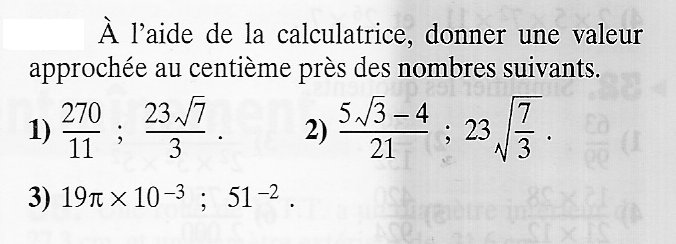
\includegraphics[width=9cm]{images/exo1.jpg}
\end{center}

\subsection*{Exercice 2}
Donnez l'�criture scientifique des nombres suivants : 

$251,3$; \enskip $0,0019$; \enskip $150$;\enskip  $150\times10^3$; \enskip
$150\times10^{-2}$; \enskip $1024$; \enskip $0,125$; \enskip $1,31\times1000$;
\enskip $18000,35$


\subsection*{Exercice 3}
\begin{center}
  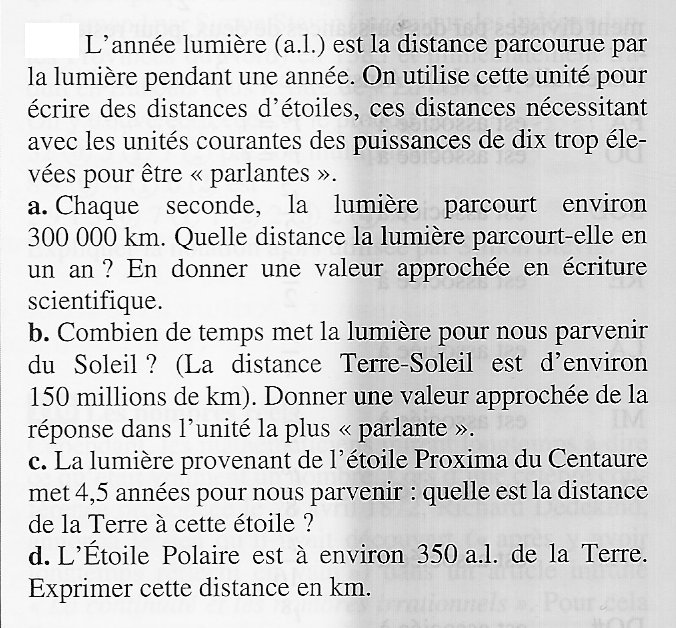
\includegraphics[width=13cm]{images/exo4.jpg}
\end{center}

\subsection*{Exercice 4}
Les nombres rationnels suivants sont-ils d�cimaux?


\bigskip
$\dfrac{-7}{523}$; \enskip $\dfrac{-17}{2000}$; \enskip $\dfrac{2}{16}$;
\enskip $\dfrac{13}{25000}$; \enskip $\dfrac{1}{28}$; 


\bigskip
En d�duire si la valeur affich�e par la calculatrice est une valeur approch�e
ou une valeur exacte du nombre.

\end{document}
